% Options for packages loaded elsewhere
\PassOptionsToPackage{unicode}{hyperref}
\PassOptionsToPackage{hyphens}{url}
\PassOptionsToPackage{dvipsnames,svgnames*,x11names*}{xcolor}
%
\documentclass[
]{memoir}
\usepackage{amsmath,amssymb}
\usepackage{lmodern}
\usepackage{ifxetex,ifluatex}
\ifnum 0\ifxetex 1\fi\ifluatex 1\fi=0 % if pdftex
  \usepackage[T1]{fontenc}
  \usepackage[utf8]{inputenc}
  \usepackage{textcomp} % provide euro and other symbols
\else % if luatex or xetex
  \usepackage{unicode-math}
  \defaultfontfeatures{Scale=MatchLowercase}
  \defaultfontfeatures[\rmfamily]{Ligatures=TeX,Scale=1}
  \setmonofont[]{Inconsolata}
\fi
% Use upquote if available, for straight quotes in verbatim environments
\IfFileExists{upquote.sty}{\usepackage{upquote}}{}
\IfFileExists{microtype.sty}{% use microtype if available
  \usepackage[]{microtype}
  \UseMicrotypeSet[protrusion]{basicmath} % disable protrusion for tt fonts
}{}
\makeatletter
\@ifundefined{KOMAClassName}{% if non-KOMA class
  \IfFileExists{parskip.sty}{%
    \usepackage{parskip}
  }{% else
    \setlength{\parindent}{0pt}
    \setlength{\parskip}{6pt plus 2pt minus 1pt}}
}{% if KOMA class
  \KOMAoptions{parskip=half}}
\makeatother
\usepackage{xcolor}
\IfFileExists{xurl.sty}{\usepackage{xurl}}{} % add URL line breaks if available
\IfFileExists{bookmark.sty}{\usepackage{bookmark}}{\usepackage{hyperref}}
\hypersetup{
  pdftitle={Data Science per psicologi},
  pdfauthor={Corrado Caudek},
  colorlinks=true,
  linkcolor=Maroon,
  filecolor=Maroon,
  citecolor=Blue,
  urlcolor=Blue,
  pdfcreator={LaTeX via pandoc}}
\urlstyle{same} % disable monospaced font for URLs
\usepackage{color}
\usepackage{fancyvrb}
\newcommand{\VerbBar}{|}
\newcommand{\VERB}{\Verb[commandchars=\\\{\}]}
\DefineVerbatimEnvironment{Highlighting}{Verbatim}{commandchars=\\\{\}}
% Add ',fontsize=\small' for more characters per line
\usepackage{framed}
\definecolor{shadecolor}{RGB}{248,248,248}
\newenvironment{Shaded}{\begin{snugshade}}{\end{snugshade}}
\newcommand{\AlertTok}[1]{\textcolor[rgb]{0.94,0.16,0.16}{#1}}
\newcommand{\AnnotationTok}[1]{\textcolor[rgb]{0.56,0.35,0.01}{\textbf{\textit{#1}}}}
\newcommand{\AttributeTok}[1]{\textcolor[rgb]{0.77,0.63,0.00}{#1}}
\newcommand{\BaseNTok}[1]{\textcolor[rgb]{0.00,0.00,0.81}{#1}}
\newcommand{\BuiltInTok}[1]{#1}
\newcommand{\CharTok}[1]{\textcolor[rgb]{0.31,0.60,0.02}{#1}}
\newcommand{\CommentTok}[1]{\textcolor[rgb]{0.56,0.35,0.01}{\textit{#1}}}
\newcommand{\CommentVarTok}[1]{\textcolor[rgb]{0.56,0.35,0.01}{\textbf{\textit{#1}}}}
\newcommand{\ConstantTok}[1]{\textcolor[rgb]{0.00,0.00,0.00}{#1}}
\newcommand{\ControlFlowTok}[1]{\textcolor[rgb]{0.13,0.29,0.53}{\textbf{#1}}}
\newcommand{\DataTypeTok}[1]{\textcolor[rgb]{0.13,0.29,0.53}{#1}}
\newcommand{\DecValTok}[1]{\textcolor[rgb]{0.00,0.00,0.81}{#1}}
\newcommand{\DocumentationTok}[1]{\textcolor[rgb]{0.56,0.35,0.01}{\textbf{\textit{#1}}}}
\newcommand{\ErrorTok}[1]{\textcolor[rgb]{0.64,0.00,0.00}{\textbf{#1}}}
\newcommand{\ExtensionTok}[1]{#1}
\newcommand{\FloatTok}[1]{\textcolor[rgb]{0.00,0.00,0.81}{#1}}
\newcommand{\FunctionTok}[1]{\textcolor[rgb]{0.00,0.00,0.00}{#1}}
\newcommand{\ImportTok}[1]{#1}
\newcommand{\InformationTok}[1]{\textcolor[rgb]{0.56,0.35,0.01}{\textbf{\textit{#1}}}}
\newcommand{\KeywordTok}[1]{\textcolor[rgb]{0.13,0.29,0.53}{\textbf{#1}}}
\newcommand{\NormalTok}[1]{#1}
\newcommand{\OperatorTok}[1]{\textcolor[rgb]{0.81,0.36,0.00}{\textbf{#1}}}
\newcommand{\OtherTok}[1]{\textcolor[rgb]{0.56,0.35,0.01}{#1}}
\newcommand{\PreprocessorTok}[1]{\textcolor[rgb]{0.56,0.35,0.01}{\textit{#1}}}
\newcommand{\RegionMarkerTok}[1]{#1}
\newcommand{\SpecialCharTok}[1]{\textcolor[rgb]{0.00,0.00,0.00}{#1}}
\newcommand{\SpecialStringTok}[1]{\textcolor[rgb]{0.31,0.60,0.02}{#1}}
\newcommand{\StringTok}[1]{\textcolor[rgb]{0.31,0.60,0.02}{#1}}
\newcommand{\VariableTok}[1]{\textcolor[rgb]{0.00,0.00,0.00}{#1}}
\newcommand{\VerbatimStringTok}[1]{\textcolor[rgb]{0.31,0.60,0.02}{#1}}
\newcommand{\WarningTok}[1]{\textcolor[rgb]{0.56,0.35,0.01}{\textbf{\textit{#1}}}}
\usepackage{longtable,booktabs,array}
\usepackage{calc} % for calculating minipage widths
% Correct order of tables after \paragraph or \subparagraph
\usepackage{etoolbox}
\makeatletter
\patchcmd\longtable{\par}{\if@noskipsec\mbox{}\fi\par}{}{}
\makeatother
% Allow footnotes in longtable head/foot
\IfFileExists{footnotehyper.sty}{\usepackage{footnotehyper}}{\usepackage{footnote}}
\makesavenoteenv{longtable}
\usepackage{graphicx}
\makeatletter
\def\maxwidth{\ifdim\Gin@nat@width>\linewidth\linewidth\else\Gin@nat@width\fi}
\def\maxheight{\ifdim\Gin@nat@height>\textheight\textheight\else\Gin@nat@height\fi}
\makeatother
% Scale images if necessary, so that they will not overflow the page
% margins by default, and it is still possible to overwrite the defaults
% using explicit options in \includegraphics[width, height, ...]{}
\setkeys{Gin}{width=\maxwidth,height=\maxheight,keepaspectratio}
% Set default figure placement to htbp
\makeatletter
\def\fps@figure{htbp}
\makeatother
\setlength{\emergencystretch}{3em} % prevent overfull lines
\providecommand{\tightlist}{%
  \setlength{\itemsep}{0pt}\setlength{\parskip}{0pt}}
\setcounter{secnumdepth}{5}
\chapterstyle{bianchi}

\usepackage{mathtools}
\usepackage[italian]{babel} 
\usepackage{booktabs}
\usepackage{hyperref}
\hypersetup{
  colorlinks=true
}
\usepackage[
  labelfont=bf, 
  font={small, it} 
]{caption} 
\usepackage{upquote} % print correct quotes in verbatim-environments
\usepackage[autostyle, italian=quotes]{csquotes}
\usepackage{empheq} 
\usepackage{xfrac}

\raggedbottom % allow variable (ragged) site heights
\frenchspacing
% \setlength\parskip{1.5pt plus 1pt minus 0.5pt}


\DeclareMathOperator{\Var}{Var} % Define variance operator
\DeclareMathOperator{\SD}{SD} % Define sd operator
\DeclareMathOperator{\Cov}{Cov} % Define covariance operator
\DeclareMathOperator{\Corr}{Corr} % Define correlation operator
\DeclareMathOperator{\Me}{Me} % Define mediane operator
\DeclareMathOperator{\Mo}{Mo} % Define mode operator
\DeclareMathOperator{\Bin}{Bin} % Define binomial operator
\DeclareMathOperator{\Bernoulli}{Bernoulli} % Define Bernoulli operator
\DeclareMathOperator{\Poi}{Poi} % Define Poisson operator
\DeclareMathOperator{\Uniform}{Uniform} % Define Uniform operator
\DeclareMathOperator{\Cauchy}{Cauchy} % Define Cauchy operator
\DeclareMathOperator{\B}{\mathscr{B}} % Define Bernoulli operator
\newcommand{\R}{\textsf{R}} % Define R programming language symbol
\newcommand{\E}{\mathbb{E}} % Define expected value operator
\newcommand{\Real}{\mathbb{R}} % Define real number operator
\newcommand{\Prob}{\mathscr{P}}
\DeclareMathOperator*{\argmin}{arg\,min} % thin space, limits on side in displays
\DeclareMathOperator*{\argmax}{arg\,max} % thin space, limits on side in displays

\usepackage{microtype}

\ifluatex
  \usepackage{selnolig}  % disable illegal ligatures
\fi
\usepackage[]{natbib}
\bibliographystyle{apalike}

\title{Data Science per psicologi}
\author{Corrado Caudek}
\date{2021-09-13}

\usepackage{amsthm}
\newtheorem{theorem}{Teorema}[chapter]
\newtheorem{lemma}{Lemma}[chapter]
\newtheorem{corollary}{Corollario}[chapter]
\newtheorem{proposition}{Proposizione}[chapter]
\newtheorem{conjecture}{Congettura}[chapter]
\theoremstyle{definition}
\newtheorem{definition}{Definizione}[chapter]
\theoremstyle{definition}
\newtheorem{example}{Esempio}[chapter]
\theoremstyle{definition}
\newtheorem{exercise}{Exercizio}[chapter]
\theoremstyle{definition}
\newtheorem{hypothesis}{Hypothesis}[chapter]
\theoremstyle{remark}
\newtheorem*{remark}{Osservazione}
\newtheorem*{solution}{Soluzione}
\begin{document}
\maketitle

{
\hypersetup{linkcolor=}
\setcounter{tocdepth}{1}
\tableofcontents
}
\newpage

\vspace*{5cm}

\thispagestyle{empty}

\hypertarget{chapter-ppc}{%
\chapter{Distribuzione predittiva a posteriori}\label{chapter-ppc}}

Oltre ad una sintesi della distribuzione a posteriori attraverso il computo di indici caratteristici e alla verifica delle ipotesi, un altro compito dell'analisi bayesiana è la predizione di nuovi dati futuri.

\begin{definition}
La \emph{distribuzione predittiva a posteriori} (\emph{posterior predictive distribution}, PPD)
\begin{equation}
p(\tilde{y} \mid y) = \int_{\theta} p(\tilde{y} \mid \theta) p(\theta \mid y) d\theta
\label{eq:dist-pred-post}
\end{equation}
\noindent
è la distribuzione di un nuovo campione di possibili osservazioni \(\tilde{Y}\) avendo già osservato \(n\) manifestazioni dello stesso fenomeno \(Y = y\).
\end{definition}

La \eqref{eq:dist-pred-post} descrive la nostra incertezza sui dati previsti futuri data la distribuzione a posteriori per \(\theta\) che abbiamo ottenuto, ovvero tenendo conto della scelta del modello e della stima dei parametri mediante i dati osservati. La distribuzione predittiva a posteriori viene usata per fare inferenze predittive, cioè per prevedere la distribuzione di nuovi dati non osservati.

\hypertarget{schema-beta-bin-distr-pred-post}{%
\section{Schema Beta-Binomiale}\label{schema-beta-bin-distr-pred-post}}

Consideriamo un'altra volta il campione di pazienti clinici depressi di \citet{zetschefuture2019} -- si veda l'Appendice \ref{es-pratico-zetsche}. Supponiamo di volere esaminare in futuro altri 20 pazienti clinici e ci chiediamo quanti di essi (\(\tilde{y} \in \{0, 1, \dots, 20\}\)) manifesteranno una depressione grave.

Se vogliamo fare predizioni su \(\tilde{y}\) dobbiamo innanzitutto riconoscere che i valori \(\tilde{y} \in [0, 20]\) non sono tutti egualmente plausibili. Sappiamo che \(\tilde{y}\) è una v.c. binomiale con distribuzione

\begin{equation}
p(\tilde{y}\mid \theta) = \binom{20}{\tilde{y}} \theta^{\tilde{y}}(1-\theta)^{20 - \tilde{y}} \; .
\label{eq:post-yprime}
\end{equation}

\noindent
La v.c. \(\tilde{y}\) dipende da \(\theta\), ma \(\theta\) è essa stessa una variabile casuale. Avendo osservato \(y = 23\) successi in \(n = 30\) prove, e avendo assunto come distribuzione a priori per \(\theta\) una \(\mbox{Beta}(2, 10)\), la distribuzione a posteriori di \(\theta\) è una \(\mbox{Beta}(25, 17)\). Per trovare la distribuzione sui possibili dati previsti futuri \(\tilde{y}\) dobbiamo dunque applicare la \eqref{eq:dist-pred-post}:

\begin{align}
p(\tilde{y} \mid y = 23) = \int_0^1 p(\tilde{y} \mid \theta) p(\theta \mid y = 23) d\theta \; .
\label{eq:post-yprime-y17}
\end{align}

Per il modello Beta-Binomiale, che stiamo discutendo, è possibile trovare una soluzione analitica all'equazione \eqref{eq:dist-pred-post}:
\begin{align}
p(\tilde{y} \mid y) &= \int_0^1 p(\tilde{y} \mid \theta)
p(\theta \mid y)\, d\theta \notag\\
 &= \int_0^1 \begin{pmatrix}\tilde{n}\\\tilde{y}\end{pmatrix}
 \theta^{\tilde{y}}
(1-\theta)^{\tilde{n}-\tilde{y}} \mbox{Beta}(a+y,b+n-y) \, d\theta \notag\\
&= \begin{pmatrix}{\tilde{n}}\\\tilde{y}\end{pmatrix} \int_0^1 \theta^{\tilde{y}}
(1-\theta)^{\tilde{n}-\tilde{y}} \frac{1}{B(a+y, b+n-y)}\theta^{a+y-1}(1-\theta)^{b+n-y-1}\notag\\
&= \begin{pmatrix}{\tilde{n}}\\\tilde{y}\end{pmatrix} \frac{1}{B(a+y, b+n-y)}\int_0^1 \theta^{\tilde{y}+a+y-1}(1-\theta)^{\tilde{n}-\tilde{y}+b+n-y-1}\notag\\
&= \begin{pmatrix}{\tilde{n}}\\\tilde{y}\end{pmatrix} \frac{B(\tilde{y}+a+y,b+n-y+\tilde{n}-\tilde{y})}{B(a+y, b+n-y)} \; .
\label{eq:post-yprime-an-sol-betabin}
\end{align}

Svolgendo i calcoli in \(\R\), per i dati dell'esempio otteniamo:

\begin{Shaded}
\begin{Highlighting}[]
\CommentTok{\# Beta Binomial Predictive distribution function}
\CommentTok{\# https://rpubs.com/FJRubio/BetaBinomialPred}
\NormalTok{BetaBinom }\OtherTok{\textless{}{-}} \FunctionTok{Vectorize}\NormalTok{(}
  \ControlFlowTok{function}\NormalTok{(rp)\{}
\NormalTok{  log\_val }\OtherTok{\textless{}{-}} \FunctionTok{lchoose}\NormalTok{(np, rp) }\SpecialCharTok{+} 
    \FunctionTok{lbeta}\NormalTok{(rp}\SpecialCharTok{+}\NormalTok{a}\SpecialCharTok{+}\NormalTok{y, b}\SpecialCharTok{+}\NormalTok{n}\SpecialCharTok{{-}}\NormalTok{y}\SpecialCharTok{+}\NormalTok{np}\SpecialCharTok{{-}}\NormalTok{rp) }\SpecialCharTok{{-}} 
    \FunctionTok{lbeta}\NormalTok{(a}\SpecialCharTok{+}\NormalTok{y, b}\SpecialCharTok{+}\NormalTok{n}\SpecialCharTok{{-}}\NormalTok{y)}
  \FunctionTok{return}\NormalTok{(}\FunctionTok{exp}\NormalTok{(log\_val))}
\NormalTok{  \}}
\NormalTok{)}

\NormalTok{n }\OtherTok{\textless{}{-}} \DecValTok{30}
\NormalTok{y }\OtherTok{\textless{}{-}} \DecValTok{23}
\NormalTok{a }\OtherTok{\textless{}{-}} \DecValTok{2}
\NormalTok{b }\OtherTok{\textless{}{-}} \DecValTok{10}
\NormalTok{np }\OtherTok{\textless{}{-}} \DecValTok{20}
\FunctionTok{data.frame}\NormalTok{(}
  \AttributeTok{heads =} \DecValTok{0}\SpecialCharTok{:}\DecValTok{20}\NormalTok{, }
  \AttributeTok{pmf =} \FunctionTok{BetaBinom}\NormalTok{(}\DecValTok{0}\SpecialCharTok{:}\DecValTok{20}\NormalTok{)}
\NormalTok{) }\SpecialCharTok{\%\textgreater{}\%}
\FunctionTok{ggplot}\NormalTok{(}\FunctionTok{aes}\NormalTok{(}\AttributeTok{x =} \FunctionTok{factor}\NormalTok{(heads), }\AttributeTok{y =}\NormalTok{ pmf)) }\SpecialCharTok{+}
  \FunctionTok{geom\_col}\NormalTok{() }\SpecialCharTok{+}
  \FunctionTok{geom\_text}\NormalTok{(}
    \FunctionTok{aes}\NormalTok{(}\AttributeTok{label =} \FunctionTok{round}\NormalTok{(pmf, }\DecValTok{2}\NormalTok{), }\AttributeTok{y =}\NormalTok{ pmf }\SpecialCharTok{+} \FloatTok{0.01}\NormalTok{),}
    \AttributeTok{position =} \FunctionTok{position\_dodge}\NormalTok{(}\FloatTok{0.9}\NormalTok{),}
    \AttributeTok{size =} \DecValTok{3}\NormalTok{,}
    \AttributeTok{vjust =} \DecValTok{0}
\NormalTok{  ) }\SpecialCharTok{+}
  \FunctionTok{labs}\NormalTok{(}
    \AttributeTok{title =} \StringTok{"Distribuzione predittiva a posteriori"}\NormalTok{,}
    \AttributeTok{x =} \StringTok{"y\textquotesingle{}"}\NormalTok{,}
    \AttributeTok{y =} \StringTok{"P(Y = y\textquotesingle{} | Data)"}
\NormalTok{  ) }
\end{Highlighting}
\end{Shaded}

\begin{center}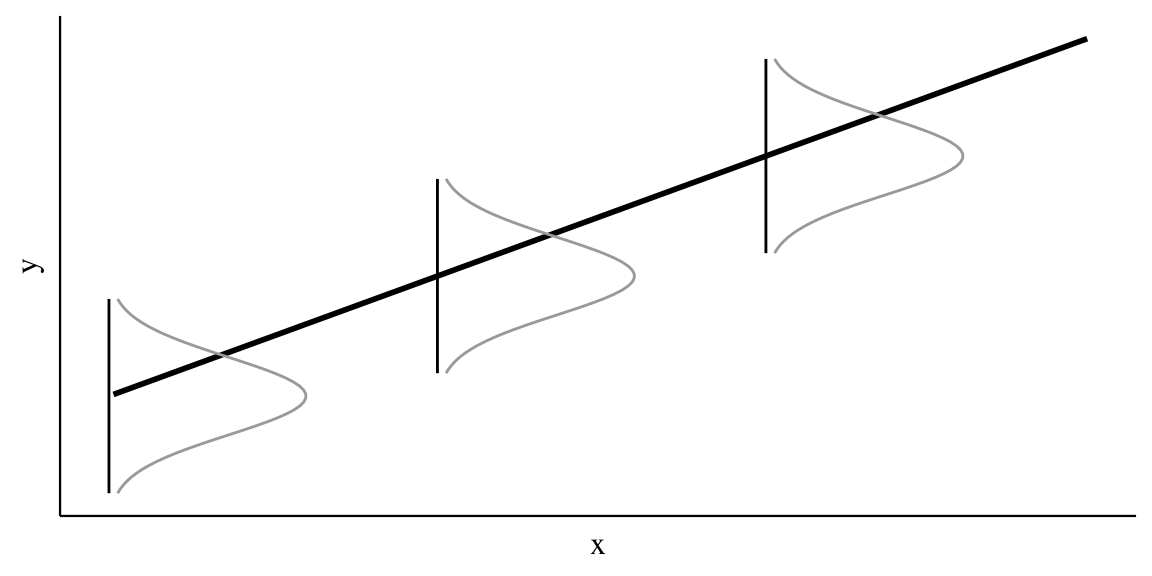
\includegraphics{046_ppc_files/figure-latex/unnamed-chunk-2-1} \end{center}

È facile vedere che, in questo esempio, la distribuzione predittiva a posteriori \(p(\tilde{y} \mid y)\) è diversa dalla binomiale di parametro \(\theta = 23/30\):

\begin{Shaded}
\begin{Highlighting}[]
\FunctionTok{tibble}\NormalTok{(}
  \AttributeTok{heads =} \DecValTok{0}\SpecialCharTok{:}\DecValTok{20}\NormalTok{, }
  \AttributeTok{pmf =} \FunctionTok{dbinom}\NormalTok{(}\AttributeTok{x =} \DecValTok{0}\SpecialCharTok{:}\DecValTok{20}\NormalTok{, }\AttributeTok{size =} \DecValTok{20}\NormalTok{, }\AttributeTok{prob =} \DecValTok{23}\SpecialCharTok{/}\DecValTok{30}\NormalTok{)}
\NormalTok{) }\SpecialCharTok{\%\textgreater{}\%}
\FunctionTok{ggplot}\NormalTok{(}\FunctionTok{aes}\NormalTok{(}\AttributeTok{x =} \FunctionTok{factor}\NormalTok{(heads), }\AttributeTok{y =}\NormalTok{ pmf)) }\SpecialCharTok{+}
  \FunctionTok{geom\_col}\NormalTok{() }\SpecialCharTok{+}
  \FunctionTok{geom\_text}\NormalTok{(}
    \FunctionTok{aes}\NormalTok{(}\AttributeTok{label =} \FunctionTok{round}\NormalTok{(pmf, }\DecValTok{2}\NormalTok{), }\AttributeTok{y =}\NormalTok{ pmf }\SpecialCharTok{+} \FloatTok{0.01}\NormalTok{),}
    \AttributeTok{position =} \FunctionTok{position\_dodge}\NormalTok{(}\FloatTok{0.9}\NormalTok{),}
    \AttributeTok{size =} \DecValTok{3}\NormalTok{,}
    \AttributeTok{vjust =} \DecValTok{0}
\NormalTok{  ) }\SpecialCharTok{+}
  \FunctionTok{labs}\NormalTok{(}\AttributeTok{title =} \StringTok{"p(y | theta = 0.77)"}\NormalTok{,}
       \AttributeTok{x =} \StringTok{"y"}\NormalTok{,}
       \AttributeTok{y =} \StringTok{"Probabilità"}\NormalTok{) }
\end{Highlighting}
\end{Shaded}

\begin{center}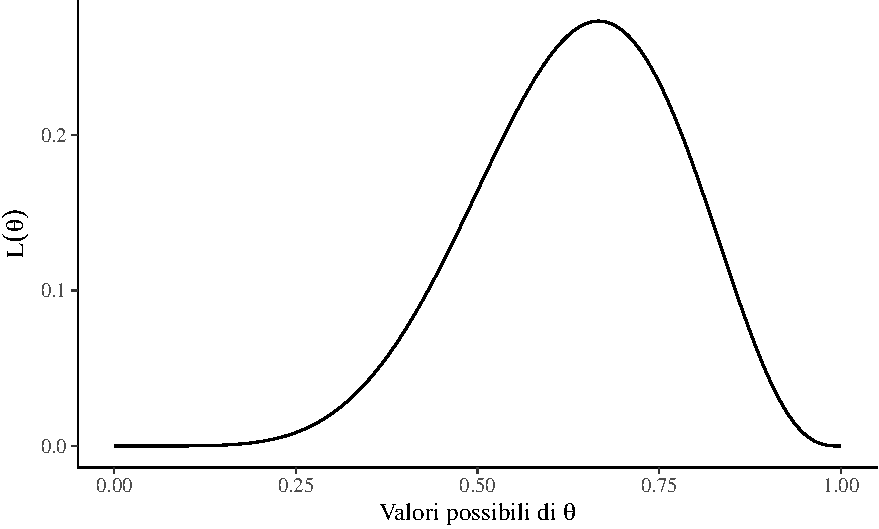
\includegraphics{046_ppc_files/figure-latex/unnamed-chunk-3-1} \end{center}

In particolare, la \(p(\tilde{y} \mid y)\) ha una varianza maggiore di \(\Bin(y \mid \theta = 0.77, n = 20)\). Questa maggiore varianza riflette le due fonti di incertezza che sono presenti nella \eqref{eq:dist-pred-post}: l'incertezza sul valore del parametro (descritta dalla distribuzione a posteriori) e l'incertezza dovuta alla variabilità campionaria (descritta dalla funzione di verosimiglianza).

Possiamo concludere la discussione di questo esempio dicendo che, nel caso di 20 nuovi pazienti clinici, ci aspettiamo di osservare 12 pazienti che manifestano una depressione severa, anche se è ragionevole aspettarci un numero compreso, diciamo, tra 8 e 16.

Una volta trovata la distribuzione predittiva a posteriori \(p(\tilde{y} \mid y)\) diventa possibile rispondere a domande come: qual è la probabilità che almeno 10 dei 20 pazienti futuri mostrino una depressione grave? Rispondere a domande di questo tipo è possibile, ma richiede un po' di lavoro --- non ci sono funzioni \(\R\) che svolgano questi calcoli per noi. Tuttavia, non è importante imparare a risolvere problemi di questo tipo perché, in generale, anche per problemi solo leggermente più complessi di quello discusso qui, non sono disponibili espressioni analitiche della distribuzione predittiva a posteriori. Mediante simulazioni MCMC, invece, è possibile trovare una approssimazione numerica della \(p(\tilde{y} \mid y)\). In tali circostanze, è più facile rispondere alle domande che ci siamo posti.

\hypertarget{metodi-mcmc-per-la-distribuzione-predittiva-a-posteriori}{%
\section{Metodi MCMC per la distribuzione predittiva a posteriori}\label{metodi-mcmc-per-la-distribuzione-predittiva-a-posteriori}}

Utilizzando la notazione di \citet{gelman2014understanding}, chiamiamo \(y^{rep}\) i dati previsti futuri che potrebbero venire osservati se l'esperimento casuale che ha prodotto \(y\) venisse ripetuto, ovvero una realizzazione futura del modello statistico con gli stessi valori dei parametri \(\theta\) che hanno prodotto \(y\). \citet{gelman2014understanding} distinguono \(y^{rep}\) (repliche sotto lo stesso modello statistico) da \(\tilde{y}\), che corrisponde invece ad un effettivo campione empirico di dati osservato in qualche futura occasione.

Mostreremo qui come ottenere \(p(y^{rep} \mid y)\) quale stima di \(p(\tilde{y} \mid y)\). Se svolgiamo l'analisi bayesiana con il metodo MCMC, \(p(y^{rep} \mid y)\) può essere ottenuta nel modo seguente:

\begin{itemize}
\tightlist
\item
  campionare \(\theta_i \sim p(\theta \mid y)\), ovvero campionare un valore del parametro dalla distribuzione a posteriori;
\item
  campionare \(y^{rep} \sim p(y^{rep} \mid \theta_i)\), ovvero campionare il valore di un'osservazione dalla funzione di verosimiglianza condizionata al valore del parametro definito nel passo precedente.
\end{itemize}

Se i due passaggi descritti sopra vengono ripetuti un numero sufficiente di volte, l'istogramma risultante approssimerà la distribuzione predittiva a posteriori che, in teoria (ma non in pratica) potrebbe essere ottenuta per via analitica (si deva il Paragrafo \ref{schema-beta-bin-distr-pred-post}).

Vediamo ora come calcolare \(p(y^{rep} \mid y)\) usando Stan. Qui di seguito è riportato il codice Stan per fare inferenza su una proporzione --- si veda il Capitolo \ref{mod-binom}:

\begin{Shaded}
\begin{Highlighting}[]
\NormalTok{modelString }\OtherTok{=} \StringTok{"}
\StringTok{data \{}
\StringTok{  int\textless{}lower=0\textgreater{} N;}
\StringTok{  int\textless{}lower=0, upper=1\textgreater{} y[N];}
\StringTok{\}}
\StringTok{parameters \{}
\StringTok{  real\textless{}lower=0, upper=1\textgreater{} theta;}
\StringTok{\}}
\StringTok{model \{}
\StringTok{  theta \textasciitilde{} beta(2, 10);}
\StringTok{  y \textasciitilde{} bernoulli(theta);}
\StringTok{\}}
\StringTok{generated quantities \{}
\StringTok{  int y\_rep[N];}
\StringTok{  real log\_lik[N];}
\StringTok{  for (n in 1:N) \{}
\StringTok{    y\_rep[n] = bernoulli\_rng(theta);}
\StringTok{    log\_lik[n] = bernoulli\_lpmf(y[n] | theta);}
\StringTok{  \}}
\StringTok{\}}
\StringTok{"}
\FunctionTok{writeLines}\NormalTok{(modelString, }\AttributeTok{con =} \StringTok{"code/betabin23{-}30{-}2{-}10.stan"}\NormalTok{)}
\end{Highlighting}
\end{Shaded}

Si noti che nel nel blocco \texttt{generated\ quantities} sono state aggiunte le istruzioni necessarie per simulare \(y^{rep}\), ovvero, \texttt{y\_rep{[}n{]}\ =\ bernoulli\_rng(theta);}.

Svolgiamo ora la simulazione. I dati dell'esempio che stiamo discutendo sono:

\begin{Shaded}
\begin{Highlighting}[]
\NormalTok{data\_list }\OtherTok{\textless{}{-}} \FunctionTok{list}\NormalTok{(}
  \AttributeTok{N =} \DecValTok{30}\NormalTok{,}
  \AttributeTok{y =} \FunctionTok{c}\NormalTok{(}\FunctionTok{rep}\NormalTok{(}\DecValTok{1}\NormalTok{, }\DecValTok{23}\NormalTok{), }\FunctionTok{rep}\NormalTok{(}\DecValTok{0}\NormalTok{, }\DecValTok{7}\NormalTok{))}
\NormalTok{)}
\end{Highlighting}
\end{Shaded}

\noindent
Compiliamo il codice Stan

\begin{Shaded}
\begin{Highlighting}[]
\NormalTok{file }\OtherTok{\textless{}{-}} \FunctionTok{file.path}\NormalTok{(}\StringTok{"code"}\NormalTok{, }\StringTok{"betabin23{-}30{-}2{-}10.stan"}\NormalTok{)}
\NormalTok{mod }\OtherTok{\textless{}{-}} \FunctionTok{cmdstan\_model}\NormalTok{(file)}
\end{Highlighting}
\end{Shaded}

\noindent
ed eseguiamo il campionamento MCMC:

\begin{Shaded}
\begin{Highlighting}[]
\NormalTok{fit }\OtherTok{\textless{}{-}}\NormalTok{ mod}\SpecialCharTok{$}\FunctionTok{sample}\NormalTok{(}
  \AttributeTok{data =}\NormalTok{ data\_list,}
  \AttributeTok{iter\_sampling =}\NormalTok{ 4000L,}
  \AttributeTok{iter\_warmup =}\NormalTok{ 2000L,}
  \AttributeTok{seed =}\NormalTok{ SEED,}
  \AttributeTok{chains =}\NormalTok{ 4L,}
  \AttributeTok{parallel\_chains =}\NormalTok{ 4L,}
  \AttributeTok{refresh =} \DecValTok{0}\NormalTok{,}
  \AttributeTok{thin =} \DecValTok{1}
\NormalTok{)}
\end{Highlighting}
\end{Shaded}

\noindent
Per comodità, trasformiamo l'oggetto \texttt{fit} in un oggetto di classe \texttt{stanfit}:

\begin{Shaded}
\begin{Highlighting}[]
\NormalTok{stanfit }\OtherTok{\textless{}{-}}\NormalTok{ rstan}\SpecialCharTok{::}\FunctionTok{read\_stan\_csv}\NormalTok{(fit}\SpecialCharTok{$}\FunctionTok{output\_files}\NormalTok{())}
\end{Highlighting}
\end{Shaded}

\noindent
Il contenuto dell'oggetto \texttt{stanfit} si può esaminare nel modo seguente:

\begin{Shaded}
\begin{Highlighting}[]
\NormalTok{list\_of\_draws }\OtherTok{\textless{}{-}} \FunctionTok{extract}\NormalTok{(stanfit)}
\FunctionTok{print}\NormalTok{(}\FunctionTok{names}\NormalTok{(list\_of\_draws))}
\CommentTok{\#\textgreater{} [1] "theta"   "y\_rep"   "log\_lik" "lp\_\_"}
\end{Highlighting}
\end{Shaded}

Occupiamoci ora della distribuzione predittiva a posteriori\footnote{Un approfondimento di questa analisi statistica è fornita nell'Appendice \ref{inference-one-prop}}. Usando l'oggetto \texttt{stanfit} creiamo \texttt{y\_bern}:

\begin{Shaded}
\begin{Highlighting}[]
\NormalTok{y\_bern }\OtherTok{\textless{}{-}}\NormalTok{ list\_of\_draws}\SpecialCharTok{$}\NormalTok{y\_rep}
\FunctionTok{dim}\NormalTok{(y\_bern)}
\CommentTok{\#\textgreater{} [1] 16000    30}
\FunctionTok{head}\NormalTok{(y\_bern)}
\CommentTok{\#\textgreater{}           }
\CommentTok{\#\textgreater{} iterations [,1] [,2] [,3] [,4] [,5] [,6] [,7] [,8] [,9]}
\CommentTok{\#\textgreater{}       [1,]    0    1    0    0    0    1    1    0    1}
\CommentTok{\#\textgreater{}       [2,]    1    0    1    1    1    1    1    1    0}
\CommentTok{\#\textgreater{}       [3,]    1    1    1    1    1    0    1    0    0}
\CommentTok{\#\textgreater{}       [4,]    1    0    0    1    1    1    0    1    1}
\CommentTok{\#\textgreater{}       [5,]    0    1    1    1    1    1    1    1    0}
\CommentTok{\#\textgreater{}       [6,]    0    0    1    1    0    1    1    0    1}
\CommentTok{\#\textgreater{}           }
\CommentTok{\#\textgreater{} iterations [,10] [,11] [,12] [,13] [,14] [,15] [,16] [,17]}
\CommentTok{\#\textgreater{}       [1,]     1     0     0     1     1     1     1     1}
\CommentTok{\#\textgreater{}       [2,]     0     0     0     1     0     1     1     1}
\CommentTok{\#\textgreater{}       [3,]     1     1     0     1     1     1     1     1}
\CommentTok{\#\textgreater{}       [4,]     1     1     0     1     0     0     0     1}
\CommentTok{\#\textgreater{}       [5,]     0     1     1     1     0     1     0     1}
\CommentTok{\#\textgreater{}       [6,]     1     0     1     0     1     1     0     0}
\CommentTok{\#\textgreater{}           }
\CommentTok{\#\textgreater{} iterations [,18] [,19] [,20] [,21] [,22] [,23] [,24] [,25]}
\CommentTok{\#\textgreater{}       [1,]     0     0     0     0     0     1     0     0}
\CommentTok{\#\textgreater{}       [2,]     1     1     1     0     1     1     0     0}
\CommentTok{\#\textgreater{}       [3,]     1     1     1     1     0     1     0     1}
\CommentTok{\#\textgreater{}       [4,]     0     0     1     1     1     1     0     0}
\CommentTok{\#\textgreater{}       [5,]     0     1     1     1     0     1     1     1}
\CommentTok{\#\textgreater{}       [6,]     1     0     0     0     0     1     0     1}
\CommentTok{\#\textgreater{}           }
\CommentTok{\#\textgreater{} iterations [,26] [,27] [,28] [,29] [,30]}
\CommentTok{\#\textgreater{}       [1,]     1     1     0     1     0}
\CommentTok{\#\textgreater{}       [2,]     0     1     1     1     0}
\CommentTok{\#\textgreater{}       [3,]     1     1     1     1     1}
\CommentTok{\#\textgreater{}       [4,]     0     0     1     0     1}
\CommentTok{\#\textgreater{}       [5,]     0     0     0     1     1}
\CommentTok{\#\textgreater{}       [6,]     1     1     0     1     1}
\end{Highlighting}
\end{Shaded}

Dato che il codice Stan definisce un modello per i dati grezzi (ovvero, per ciascuna singola prova Bernoulliana del campione), ogni riga di \texttt{y\_bern} include 30 colonne, ciascuna delle quali è una stima di un nuovo futuro valore possibile \(y_i \in \{0, 1\}\). Per ottenere \texttt{y\_rep}, ovvero, il numero previsto di ``successi'' in nuove future \(N = 30\) prove è sufficiente calcolare la somma dei valori di ciascuna riga. Ripetendo questa operazione per tutte le 16000 righe otteniamo una stima della distribuzione predittiva a posteriori:

\begin{Shaded}
\begin{Highlighting}[]
\FunctionTok{data.frame}\NormalTok{(}\AttributeTok{y\_rep =} \FunctionTok{rowSums}\NormalTok{(y\_bern)) }\SpecialCharTok{\%\textgreater{}\%} 
  \FunctionTok{ggplot}\NormalTok{(}\FunctionTok{aes}\NormalTok{(}\AttributeTok{x =}\NormalTok{ y\_rep)) }\SpecialCharTok{+} 
  \FunctionTok{stat\_count}\NormalTok{()}
\end{Highlighting}
\end{Shaded}

\begin{center}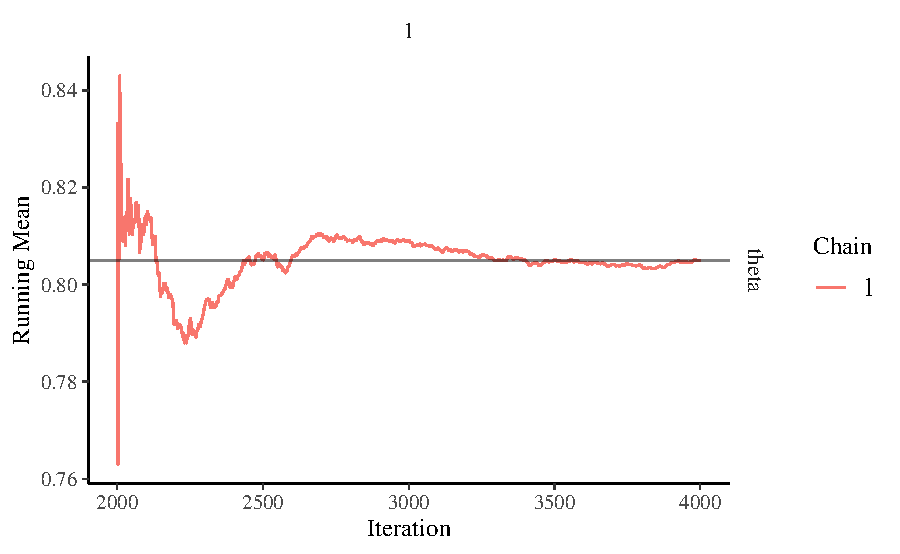
\includegraphics{046_ppc_files/figure-latex/unnamed-chunk-11-1} \end{center}

Si noti che la simulazione di \texttt{y\_rep} assume che l'ampiezza del campione di dati futuri sia uguale all'ampiezza del campione di dati osservati --- nel caso presente \(n = 30\).

\hypertarget{posterior-predictive-checks}{%
\section{Posterior predictive checks}\label{posterior-predictive-checks}}

La distribuzione predittiva a posteriori viene utilizzata per eseguire i cosiddetti \emph{Posterior Predictive Checks} (PPC). I PPC vengono utilizzati per valutare l'\emph{accuratezza predittiva} del modello, ovvero per confrontare con metodi grafici la distribuzione dei dati osservati \(y\) con la stima della distribuzione predittiva a posteriori \(p(y^{rep} \mid y)\). Confrontando visivamente gli aspetti chiave dei dati previsti futuri \(y^{rep}\) e dei dati osservati \(y\) possiamo determinare se il modello è adeguato. Se il modello si adatta bene ai dati, la distribuzione di \(y^{rep}\) è molto simile alla distribuzione dei dati osservati. In altre parole, i dati osservati devono risultare plausibili alla luce della distribuzione predittiva a posteriori.

Oltre al confronto tra le distribuzioni di \(y\) e di \(y^{rep}\) è anche possibile un confronto tra la distribuzione di varie statistiche descrittive, i cui valori sono calcolati su diversi campioni \(y^{rep}\), e le corrispondenti statistiche descrittive calcolate sui dati osservati. Vengono solitamente considerate statistiche descrittive quali la media, la varianza, la deviazione standard, il minimo o il massimo. Ma confronti di questo tipo sono possibili per qualunque statistica descrittiva. Questi confronti sono appunto chiamati PPC.

Per l'esempio presente, una volta eseguito il campionamento MCMC e ottenuto un oggetto di classe \texttt{stanfit}, è possibile usare le funzionalità del pacchetto \texttt{bayesplot} per eseguire i PPC. Nel caso presente, il campione di dati ha dimensioni esigue, per cui i PPC rifletteranno la grande incertenzza dell'inferenza.

Dall'oggetto \texttt{stanfit} estraiamo \(y^{rep}\):

\begin{Shaded}
\begin{Highlighting}[]
\NormalTok{y\_rep }\OtherTok{\textless{}{-}} \FunctionTok{as.matrix}\NormalTok{(stanfit, }\AttributeTok{pars =} \StringTok{"y\_rep"}\NormalTok{)}
\FunctionTok{dim}\NormalTok{(y\_rep)}
\CommentTok{\#\textgreater{} [1] 16000    30}
\end{Highlighting}
\end{Shaded}

\noindent
Qui sotto esaminiamo la distribuzione della \(y\) insieme alla distribuzione di 8 campioni \(y^{rep}\):

\begin{Shaded}
\begin{Highlighting}[]
\FunctionTok{ppc\_hist}\NormalTok{(data\_list}\SpecialCharTok{$}\NormalTok{y, y\_rep[}\DecValTok{1}\SpecialCharTok{:}\DecValTok{8}\NormalTok{, ], }\AttributeTok{binwidth =} \DecValTok{1}\NormalTok{)}
\end{Highlighting}
\end{Shaded}

\begin{center}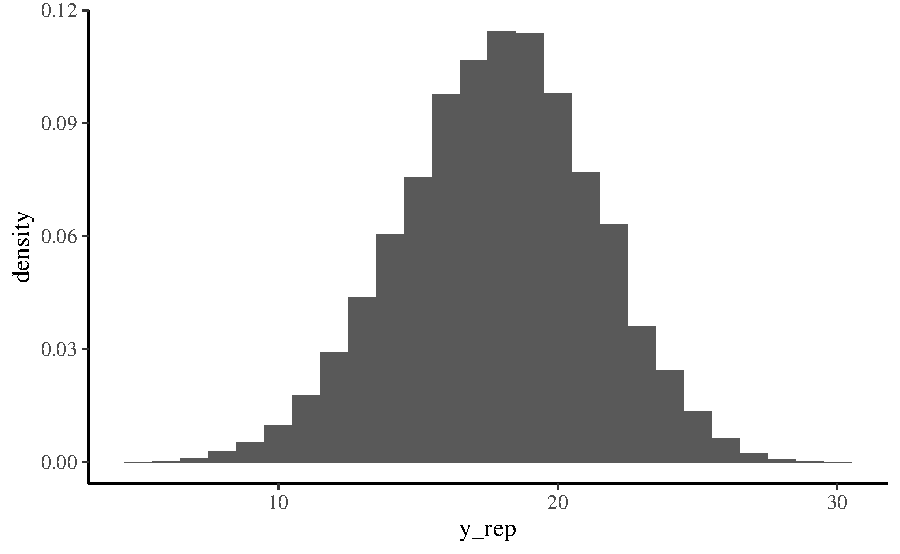
\includegraphics{046_ppc_files/figure-latex/unnamed-chunk-13-1} \end{center}

La corrispondenza tra le distribuzioni della \(y\) e di \(y^{rep}\) è solo parziale. Il confronto è più facile se sovrapponiamo graficamente i kernel density plot della \(y\) e di \(y^{rep}\) (qui usiamo 50 campioni \(y^{rep}\)):

\begin{Shaded}
\begin{Highlighting}[]
\FunctionTok{ppc\_dens\_overlay}\NormalTok{(data\_list}\SpecialCharTok{$}\NormalTok{y, y\_rep[}\DecValTok{1}\SpecialCharTok{:}\DecValTok{50}\NormalTok{, ])}
\end{Highlighting}
\end{Shaded}

\begin{center}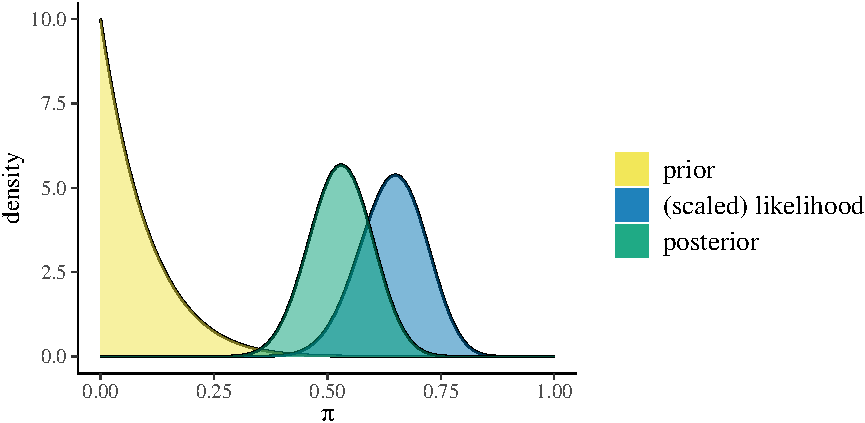
\includegraphics{046_ppc_files/figure-latex/unnamed-chunk-14-1} \end{center}

Anche in questo caso c'è una corrispondenza solo approssimativa tra l'istogramma lisciato della \(y\) e quello di \(y^{rep}\) --- ciò è dovuto al fatto che il campione è molto piccolo.

La distribuzione predittiva a posteriori è comunque in grado di rappresentare abbastanza bene la media di \(y\):

\begin{Shaded}
\begin{Highlighting}[]
\FunctionTok{ppc\_stat}\NormalTok{(data\_list}\SpecialCharTok{$}\NormalTok{y, y\_rep, }\AttributeTok{stat =} \StringTok{"mean"}\NormalTok{)}
\end{Highlighting}
\end{Shaded}

\begin{center}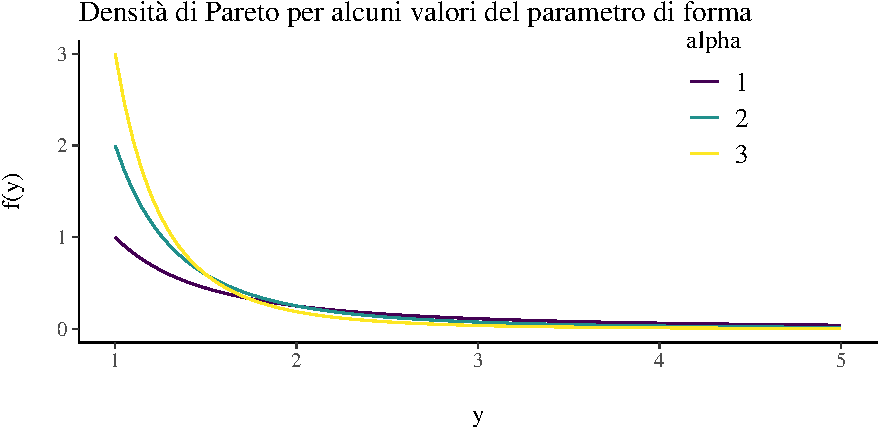
\includegraphics{046_ppc_files/figure-latex/unnamed-chunk-15-1} \end{center}

\noindent
Lo stesso si può dire della varianza:

\begin{Shaded}
\begin{Highlighting}[]
\FunctionTok{ppc\_stat}\NormalTok{(data\_list}\SpecialCharTok{$}\NormalTok{y, y\_rep, }\AttributeTok{stat =} \StringTok{"var"}\NormalTok{)}
\end{Highlighting}
\end{Shaded}

\begin{center}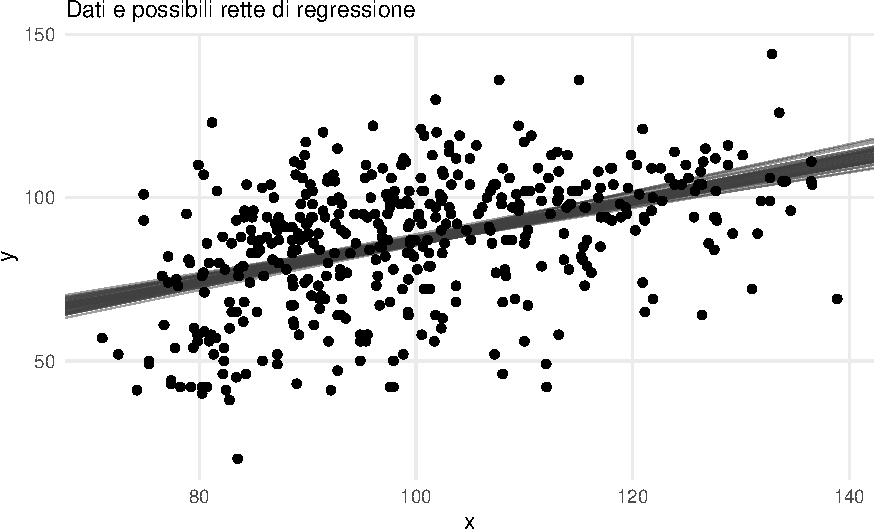
\includegraphics{046_ppc_files/figure-latex/unnamed-chunk-16-1} \end{center}

Nell'esempio successivo considereremo un campione più grande e vedremo come i PPC possano fornirci delle indicazioni sulla mancanza di adattamento del modello ai dati.

\hypertarget{ppc-per-il-modello-di-poisson}{%
\subsection{PPC per il modello di Poisson}\label{ppc-per-il-modello-di-poisson}}

Le istruzioni \(\R\) qui utilizzate sono state recuperate dalla seguente \href{http://avehtari.github.io/BDA_R_demos/demos_rstan/ppc/poisson-ppc.html\#}{pagina web}. Nell'esempio discusso da Jonah Gabry e Aki Vehtari vengono usati i seguenti dati:

\begin{Shaded}
\begin{Highlighting}[]
\NormalTok{y }\OtherTok{\textless{}{-}} \FunctionTok{c}\NormalTok{(0L, 3L, 5L, 0L, 4L, 7L, 4L, 2L, 3L, }
\NormalTok{       6L, 7L, 0L, 0L, 3L, 7L, 5L, 5L, 0L, }
\NormalTok{       4L, 0L, 4L, 4L, 6L, 3L, 7L, 5L, 3L, }
\NormalTok{       0L, 0L, 2L, 0L, 1L, 0L, 1L, 5L, 4L, }
\NormalTok{       4L, 2L, 3L, 6L, 4L, 5L, 0L, 7L, 7L, }
\NormalTok{       4L, 4L, 4L, 0L, 6L, 1L, 5L, 6L, 5L, }
\NormalTok{       6L, 7L, 3L, 6L, 2L, 3L, 0L, 2L, 0L, }
\NormalTok{       6L, 6L, 0L, 3L, 4L, 4L, 5L, 5L, 0L, }
\NormalTok{       5L, 7L, 5L, 5L, 6L, 4L, 2L, 3L, 4L, }
\NormalTok{       6L, 4L, 6L, 6L, 4L, 0L, 6L, 5L, 5L, }
\NormalTok{       7L, 0L, 1L, 6L, 7L, 0L, 5L, 0L, 0L, }
\NormalTok{       5L, 6L, 5L, 1L, 0L, 7L, 1L, 2L, 6L, }
\NormalTok{       5L, 4L, 0L, 4L, 0L, 4L, 4L, 6L, 3L, }
\NormalTok{       0L, 0L, 3L, 3L, 4L, 2L, 5L, 3L, 4L, }
\NormalTok{       3L, 2L, 5L, 2L, 4L, 4L, 0L, 2L, 7L, }
\NormalTok{       5L, 7L, 5L, 5L, 7L, 7L, 0L, 4L, 6L, }
\NormalTok{       0L, 4L, 6L, 7L, 4L, 0L, 4L, 1L, 5L, }
\NormalTok{       0L, 3L, 5L, 7L, 6L, 0L, 5L, 5L, 6L, }
\NormalTok{       7L, 6L, 7L, 3L, 4L, 3L, 7L, 7L, 2L, }
\NormalTok{       5L, 4L, 5L, 5L, 0L, 6L, 2L, 4L, 5L, }
\NormalTok{       4L, 0L, 0L, 5L, 5L, 7L, 7L, 0L, 3L, }
\NormalTok{       0L, 3L, 3L, 6L, 1L, 4L, 2L, 0L, 4L, }
\NormalTok{       7L, 5L, 5L, 0L, 3L, 7L, 0L, 6L, 6L, }
\NormalTok{       4L, 1L, 6L, 7L, 6L, 0L, 3L, 6L, 4L, }
\NormalTok{       7L, 0L, 5L, 5L, 4L, 0L, 0L, 2L, 4L, }
\NormalTok{       6L, 0L, 5L, 0L, 2L, 7L, 2L, 7L, 5L, }
\NormalTok{       4L, 6L, 2L, 4L, 0L, 4L, 0L, 0L, 3L, }
\NormalTok{       5L, 4L, 3L, 5L, 5L, 7L, 7L, 0L, 6L, }
\NormalTok{       4L, 5L, 1L, 5L, 3L, 5L, 5L, 5L, 0L, }
\NormalTok{       2L, 7L, 6L, 2L, 3L, 2L, 5L, 4L, 7L, }
\NormalTok{       6L, 7L, 3L, 3L, 4L, 4L, 6L, 4L, 6L, }
\NormalTok{       7L, 1L, 5L, 6L, 3L, 3L, 6L, 3L, 4L, }
\NormalTok{       0L, 7L, 0L, 3L, 6L, 5L, 0L, 0L, 0L, }
\NormalTok{       5L, 4L, 4L, 0L, 4L, 7L, 5L, 5L, 3L, }
\NormalTok{       3L, 0L, 0L, 5L, 4L, 0L, 7L, 6L, 0L, }
\NormalTok{       6L, 2L, 0L, 6L, 1L, 0L, 4L, 0L, 4L, }
\NormalTok{       3L, 0L, 4L, 5L, 5L, 7L, 6L, 6L, 5L, }
\NormalTok{       4L, 7L, 0L, 6L, 4L, 7L, 7L, 5L, 0L, }
\NormalTok{       1L, 4L, 7L, 6L, 4L, 5L, 4L, 7L, 2L, }
\NormalTok{       5L, 2L, 6L, 3L, 2L, 7L, 4L, 3L, 4L, }
\NormalTok{       6L, 6L, 6L, 6L, 7L, 1L, 0L, 0L, 7L, }
\NormalTok{       7L, 4L, 2L, 4L, 5L, 5L, 7L, 4L, 1L, }
\NormalTok{       7L, 6L, 5L, 6L, 5L, 4L, 0L, 0L, 7L, }
\NormalTok{       0L, 0L, 5L, 6L, 6L, 3L, 6L, 0L, 0L, }
\NormalTok{       0L, 4L, 4L, 3L, 0L, 7L, 5L, 4L, 2L, }
\NormalTok{       7L, 0L, 4L, 0L, 0L, 2L, 4L, 5L, 0L, }
\NormalTok{       4L, 2L, 5L, 2L, 0L, 6L, 6L, 3L, 6L, }
\NormalTok{       0L, 2L, 5L, 0L, 0L, 0L, 6L, 0L, 0L, }
\NormalTok{       6L, 5L, 4L, 6L, 4L, 5L, 5L, 4L, 0L, }
\NormalTok{       3L, 4L, 3L, 3L, 5L, 3L, 4L, 5L, 7L, }
\NormalTok{       0L, 0L, 1L, 4L, 6L, 3L, 5L, 7L, 6L, }
\NormalTok{       6L, 5L, 0L, 5L, 4L, 0L, 0L, 2L, 6L, }
\NormalTok{       0L, 6L, 0L, 4L, 5L, 6L, 3L, 4L, 2L, }
\NormalTok{       3L, 4L, 0L, 5L, 0L, 0L, 0L, 0L, 3L, }
\NormalTok{       4L, 7L, 6L, 7L, 7L, 3L, 4L, 4L, 7L, }
\NormalTok{       4L, 5L, 2L, 5L, 6L)}

\NormalTok{N }\OtherTok{\textless{}{-}} \FunctionTok{length}\NormalTok{(y)}
\end{Highlighting}
\end{Shaded}

\noindent
Per questi dati sembra appropriato un modello di Poisson.

\begin{Shaded}
\begin{Highlighting}[]
\FunctionTok{qplot}\NormalTok{(y)}
\end{Highlighting}
\end{Shaded}

\begin{center}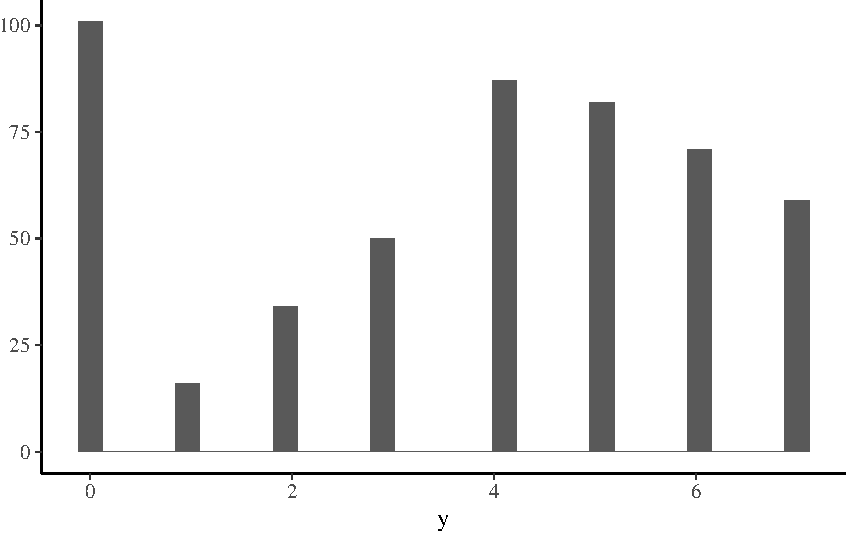
\includegraphics{046_ppc_files/figure-latex/unnamed-chunk-18-1} \end{center}

\noindent
Un istogramma di un campione casuale della stessa ampiezza di \(y\) tratto dalla distribuzione di Poisson è il seguente:

\begin{Shaded}
\begin{Highlighting}[]
\NormalTok{x }\OtherTok{\textless{}{-}} \FunctionTok{rpois}\NormalTok{(N, }\FunctionTok{mean}\NormalTok{(y))}
\FunctionTok{qplot}\NormalTok{(x)}
\end{Highlighting}
\end{Shaded}

\begin{center}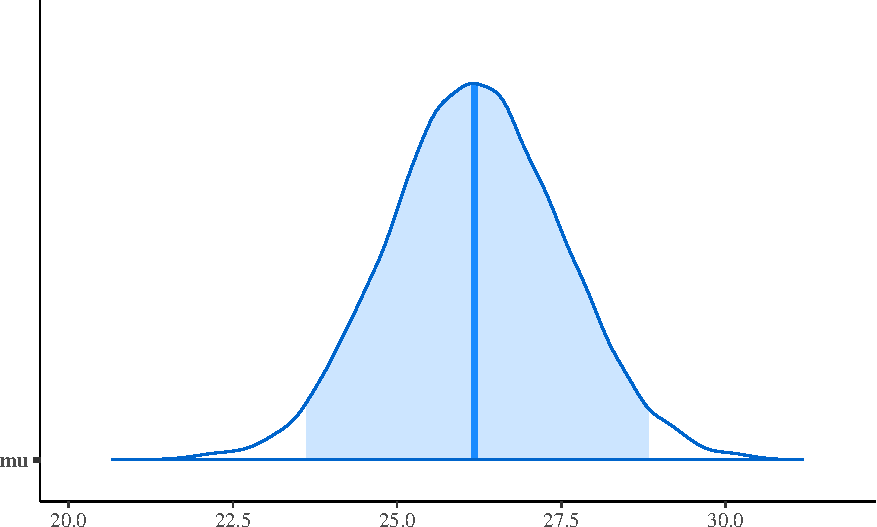
\includegraphics{046_ppc_files/figure-latex/unnamed-chunk-19-1} \end{center}

\noindent
È chiaro però che i due istogrammi sono molto diversi.

Anche se sospettiamo che non sarà un buon modello per questi dati, è comunque una buona idea iniziare adattando ai dati il modello più semplice, ovvero quello di Poisson. Partendo da lì possiamo poi cercare di capire in che modo il modello è inadeguato.

\begin{Shaded}
\begin{Highlighting}[]
\NormalTok{modelString }\OtherTok{\textless{}{-}} \StringTok{"}
\StringTok{data \{}
\StringTok{  int\textless{}lower=1\textgreater{} N;}
\StringTok{  int\textless{}lower=0\textgreater{} y[N];}
\StringTok{\}}
\StringTok{parameters \{}
\StringTok{  real\textless{}lower=0\textgreater{} lambda;}
\StringTok{\}}
\StringTok{model \{}
\StringTok{  lambda \textasciitilde{} exponential(0.2);}
\StringTok{  y \textasciitilde{} poisson(lambda);}
\StringTok{\}}
\StringTok{generated quantities \{}
\StringTok{  int y\_rep[N];}
\StringTok{  for (n in 1:N) \{}
\StringTok{    y\_rep[n] = poisson\_rng(lambda);}
\StringTok{  \}}
\StringTok{\}}
\StringTok{"}
\FunctionTok{writeLines}\NormalTok{(modelString, }\AttributeTok{con =} \StringTok{"code/code\_poisson.stan"}\NormalTok{)}
\end{Highlighting}
\end{Shaded}

\noindent
Creiamo un oggetto di tipo \texttt{list} dove inserire i dati:

\begin{Shaded}
\begin{Highlighting}[]
\NormalTok{data\_list }\OtherTok{\textless{}{-}} \FunctionTok{list}\NormalTok{(}
  \AttributeTok{y =}\NormalTok{ y,}
  \AttributeTok{N =} \FunctionTok{length}\NormalTok{(y)}
\NormalTok{)}
\end{Highlighting}
\end{Shaded}

\noindent
Adattando il modello ai dati

\begin{Shaded}
\begin{Highlighting}[]
\NormalTok{file }\OtherTok{\textless{}{-}} \FunctionTok{file.path}\NormalTok{(}\StringTok{"code"}\NormalTok{, }\StringTok{"code\_poisson.stan"}\NormalTok{)}
\NormalTok{mod }\OtherTok{\textless{}{-}} \FunctionTok{cmdstan\_model}\NormalTok{(file)}
\NormalTok{fit }\OtherTok{\textless{}{-}}\NormalTok{ mod}\SpecialCharTok{$}\FunctionTok{sample}\NormalTok{(}
  \AttributeTok{data =}\NormalTok{ data\_list,}
  \AttributeTok{iter\_sampling =}\NormalTok{ 4000L,}
  \AttributeTok{iter\_warmup =}\NormalTok{ 2000L,}
  \AttributeTok{seed =}\NormalTok{ SEED,}
  \AttributeTok{chains =}\NormalTok{ 4L,}
  \AttributeTok{parallel\_chains =}\NormalTok{ 4L,}
  \AttributeTok{refresh =} \DecValTok{0}\NormalTok{,}
  \AttributeTok{thin =} \DecValTok{1}
\NormalTok{)}
\end{Highlighting}
\end{Shaded}

\noindent
otteniamo la seguente stima del parametro \(\lambda\):

\begin{Shaded}
\begin{Highlighting}[]
\NormalTok{fit}\SpecialCharTok{$}\FunctionTok{summary}\NormalTok{(}\FunctionTok{c}\NormalTok{(}\StringTok{"lambda"}\NormalTok{))}
\CommentTok{\#\textgreater{} \# A tibble: 1 x 10}
\CommentTok{\#\textgreater{}   variable  mean median     sd    mad    q5   q95  rhat}
\CommentTok{\#\textgreater{}   \textless{}chr\textgreater{}    \textless{}dbl\textgreater{}  \textless{}dbl\textgreater{}  \textless{}dbl\textgreater{}  \textless{}dbl\textgreater{} \textless{}dbl\textgreater{} \textless{}dbl\textgreater{} \textless{}dbl\textgreater{}}
\CommentTok{\#\textgreater{} 1 lambda    3.66   3.66 0.0839 0.0837  3.52  3.80  1.00}
\CommentTok{\#\textgreater{} \# ... with 2 more variables: ess\_bulk \textless{}dbl\textgreater{}, ess\_tail \textless{}dbl\textgreater{}}
\end{Highlighting}
\end{Shaded}

\noindent
Confrontiamo \(\lambda\) con la media di \(y\):

\begin{Shaded}
\begin{Highlighting}[]
\FunctionTok{mean}\NormalTok{(y)}
\CommentTok{\#\textgreater{} [1] 3.662}
\end{Highlighting}
\end{Shaded}

Anche se trova la media giusta, il modello non è comunque adeguato a prevedere le altre proprietà della \(y\). Trasformiamo \texttt{fit} in un oggetto \texttt{stanfit}:

\begin{Shaded}
\begin{Highlighting}[]
\NormalTok{stanfit }\OtherTok{\textless{}{-}}\NormalTok{ rstan}\SpecialCharTok{::}\FunctionTok{read\_stan\_csv}\NormalTok{(fit}\SpecialCharTok{$}\FunctionTok{output\_files}\NormalTok{())}
\end{Highlighting}
\end{Shaded}

\noindent
La distribuzione a posteriori di \(\lambda\) è

\begin{Shaded}
\begin{Highlighting}[]
\NormalTok{lambda\_draws }\OtherTok{\textless{}{-}} \FunctionTok{as.matrix}\NormalTok{(stanfit, }\AttributeTok{pars =} \StringTok{"lambda"}\NormalTok{)}
\FunctionTok{mcmc\_areas}\NormalTok{(lambda\_draws, }\AttributeTok{prob =} \FloatTok{0.95}\NormalTok{) }\CommentTok{\# color 95\% interval}
\end{Highlighting}
\end{Shaded}

\begin{center}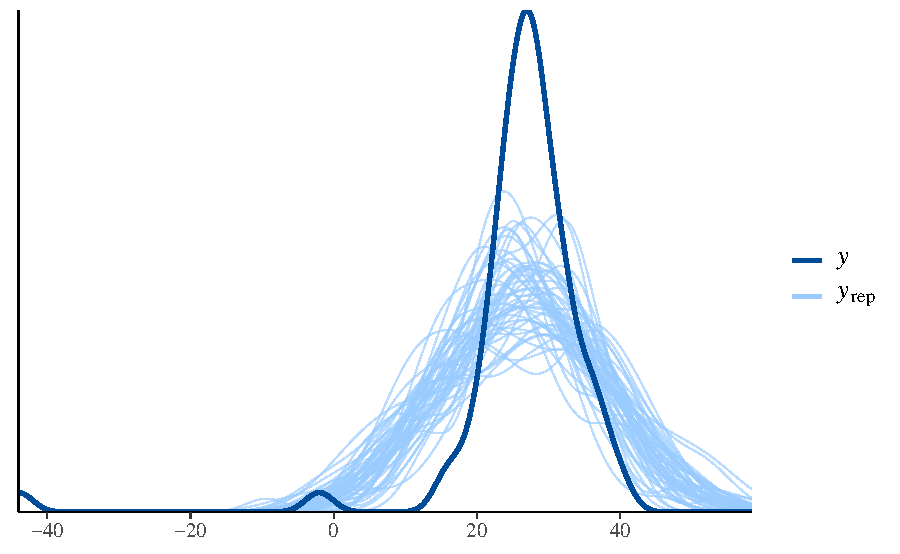
\includegraphics{046_ppc_files/figure-latex/unnamed-chunk-26-1} \end{center}

\noindent
Estraiamo \(y^{rep}\) dall'oggetto \texttt{stanfit}:

\begin{Shaded}
\begin{Highlighting}[]
\NormalTok{y\_rep }\OtherTok{\textless{}{-}} \FunctionTok{as.matrix}\NormalTok{(stanfit, }\AttributeTok{pars =} \StringTok{"y\_rep"}\NormalTok{)}
\FunctionTok{dim}\NormalTok{(y\_rep) }
\CommentTok{\#\textgreater{} [1] 16000   500}
\end{Highlighting}
\end{Shaded}

Il confronto tra l'istogramma della \(y\) e gli istogrammi di diversi campioni \(y^{rep}\) mostra una scarsa corrispondenza tra i due:

\begin{Shaded}
\begin{Highlighting}[]
\FunctionTok{ppc\_hist}\NormalTok{(y, y\_rep[}\DecValTok{1}\SpecialCharTok{:}\DecValTok{8}\NormalTok{, ], }\AttributeTok{binwidth =} \DecValTok{1}\NormalTok{)}
\end{Highlighting}
\end{Shaded}

\begin{center}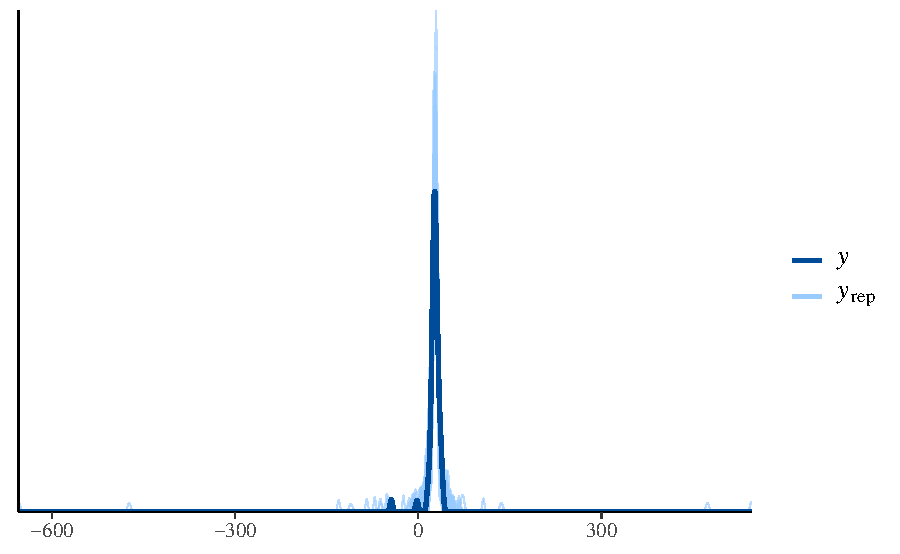
\includegraphics{046_ppc_files/figure-latex/unnamed-chunk-28-1} \end{center}

Alla stessa conclusione si giunge tramite un confronto tra la funzione di densità empirica della \(y\) e quella di diversi campioni \(y^{rep}\):

\begin{Shaded}
\begin{Highlighting}[]
\FunctionTok{ppc\_dens\_overlay}\NormalTok{(y, y\_rep[}\DecValTok{1}\SpecialCharTok{:}\DecValTok{50}\NormalTok{, ])}
\end{Highlighting}
\end{Shaded}

\begin{center}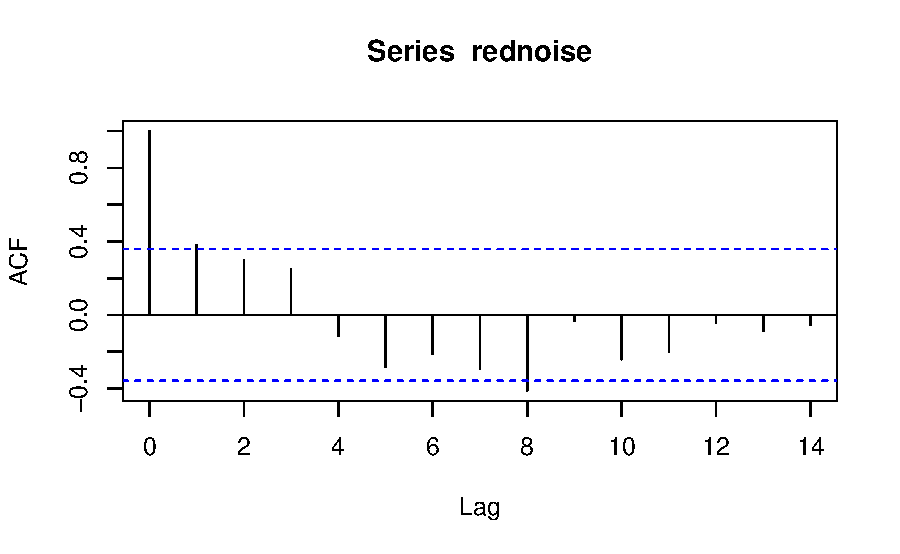
\includegraphics{046_ppc_files/figure-latex/unnamed-chunk-29-1} \end{center}

Eseguiamo ora i PPC per la media e la deviazine standard:

\begin{Shaded}
\begin{Highlighting}[]
\FunctionTok{ppc\_stat\_2d}\NormalTok{(y, y\_rep, }\AttributeTok{stat =} \FunctionTok{c}\NormalTok{(}\StringTok{"mean"}\NormalTok{, }\StringTok{"sd"}\NormalTok{))}
\end{Highlighting}
\end{Shaded}

\begin{center}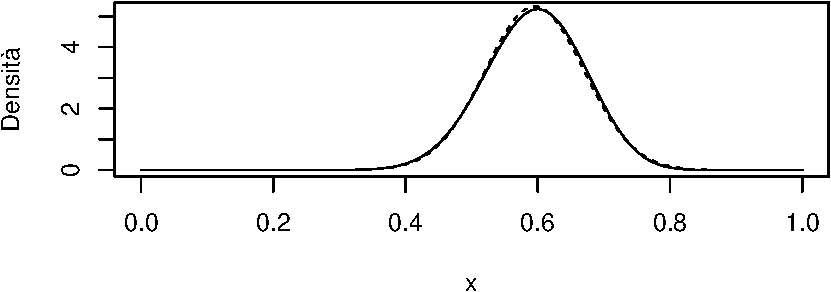
\includegraphics{046_ppc_files/figure-latex/unnamed-chunk-30-1} \end{center}

\noindent
Mentre la media viene riprodotta accuratamente dal modello (come avevamo visto sopra), ciò non è vero per la deviazione stanard dei dati. La domanda è quale sia l'origine di questa mancanza di adattamento.

Calcoliamo ora la proporzione di zeri in \(y\) e nei campioni \(y^{rep}\).

\begin{Shaded}
\begin{Highlighting}[]
\NormalTok{prop\_zero }\OtherTok{\textless{}{-}} \ControlFlowTok{function}\NormalTok{(x) }\FunctionTok{mean}\NormalTok{(x }\SpecialCharTok{==} \DecValTok{0}\NormalTok{)}
\FunctionTok{print}\NormalTok{(}\FunctionTok{prop\_zero}\NormalTok{(y))}
\CommentTok{\#\textgreater{} [1] 0.202}
\end{Highlighting}
\end{Shaded}

Eseguendo il PPC sulla proporzione di zeri

\begin{Shaded}
\begin{Highlighting}[]
\FunctionTok{ppc\_stat}\NormalTok{(y, y\_rep, }\AttributeTok{stat =} \StringTok{"prop\_zero"}\NormalTok{)}
\end{Highlighting}
\end{Shaded}

\begin{center}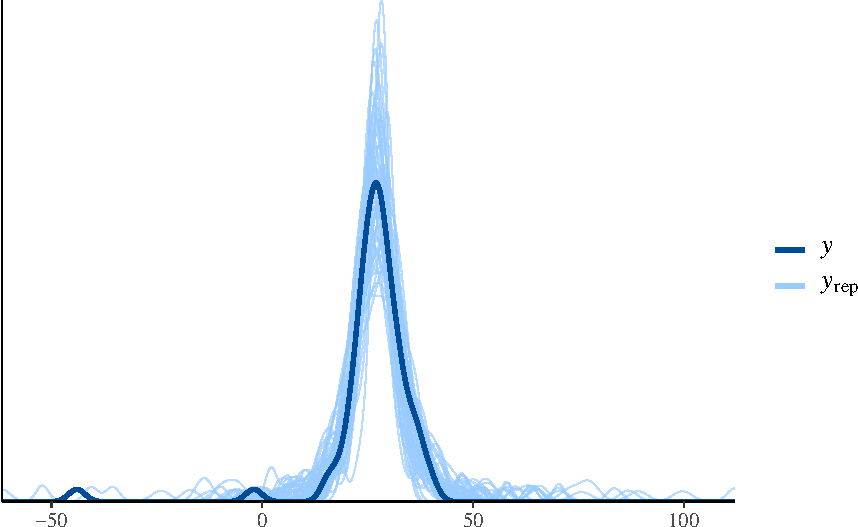
\includegraphics{046_ppc_files/figure-latex/unnamed-chunk-32-1} \end{center}

\noindent 
notiamo che il modello non è assolutamente in grado di catturare la proporzione di casi nei quali la variabile \(Y\) assume il valore 0. In altri termini, i dati presentano un'inflazione di valori 0 rispetto a quelli che sono previsti da un modello di Poisson. Questo è un problema che si verifica spesso nei dati empirici.

Per ovviare al problema dell'inflazione di valori pari a 0 è possibile definire un modello di tipo ``hurdle'' che consente la presenza di una proporzione di valori pari a 0 maggiore di quanto normalmente previsto dalla distribuzione di Poisson. Senza entrare nei dettagli di come questo viene fatto, Gabry e Vehtari definiscono il seguente modello:

\begin{Shaded}
\begin{Highlighting}[]
\NormalTok{modelString2 }\OtherTok{\textless{}{-}} \StringTok{"}
\StringTok{data \{}
\StringTok{  int\textless{}lower=1\textgreater{} N;}
\StringTok{  int\textless{}lower=0\textgreater{} y[N];}
\StringTok{\}}
\StringTok{transformed data \{}
\StringTok{  int U = max(y);  // upper truncation point}
\StringTok{\}}
\StringTok{parameters \{}
\StringTok{  real\textless{}lower=0,upper=1\textgreater{} theta; // Pr(y = 0)}
\StringTok{  real\textless{}lower=0\textgreater{} lambda; // Poisson rate parameter (if y \textgreater{} 0)}
\StringTok{\}}
\StringTok{model \{}
\StringTok{  lambda \textasciitilde{} exponential(0.2);}
\StringTok{  }
\StringTok{  for (n in 1:N) \{}
\StringTok{    if (y[n] == 0) \{}
\StringTok{      target += log(theta);  // log(Pr(y = 0))}
\StringTok{    \} else \{}
\StringTok{      target += log1m(theta);  // log(Pr(y \textgreater{} 0))}
\StringTok{      y[n] \textasciitilde{} poisson(lambda) T[1,U];  // truncated poisson}
\StringTok{    \}}
\StringTok{  \}}
\StringTok{\}}
\StringTok{generated quantities \{}
\StringTok{  real log\_lik[N];}
\StringTok{  int y\_rep[N];}
\StringTok{  for (n in 1:N) \{}
\StringTok{    if (bernoulli\_rng(theta)) \{}
\StringTok{      y\_rep[n] = 0;}
\StringTok{    \} else \{}
\StringTok{      int w;  // temporary variable}
\StringTok{      w = poisson\_rng(lambda); }
\StringTok{      while (w == 0 || w \textgreater{} U)}
\StringTok{        w = poisson\_rng(lambda);}
\StringTok{        }
\StringTok{      y\_rep[n] = w;}
\StringTok{    \}}
\StringTok{    if (y[n] == 0) \{}
\StringTok{      log\_lik[n] = log(theta);}
\StringTok{    \} else \{}
\StringTok{      log\_lik[n] = log1m(theta)}
\StringTok{    + poisson\_lpmf(y[n] | lambda)}
\StringTok{    {-} log\_diff\_exp(poisson\_lcdf(U | lambda),}
\StringTok{                       poisson\_lcdf(0 | lambda));}
\StringTok{    \}}
\StringTok{  \}}
\StringTok{\}}
\StringTok{"}
\FunctionTok{writeLines}\NormalTok{(modelString2, }\AttributeTok{con =} \StringTok{"code/code\_poisson\_hurdle.stan"}\NormalTok{)}
\end{Highlighting}
\end{Shaded}

\noindent
Adattiamo il modello ai dati:

\begin{Shaded}
\begin{Highlighting}[]
\NormalTok{file2 }\OtherTok{\textless{}{-}} \FunctionTok{file.path}\NormalTok{(}\StringTok{"code"}\NormalTok{, }\StringTok{"code\_poisson\_hurdle.stan"}\NormalTok{)}
\NormalTok{mod2 }\OtherTok{\textless{}{-}} \FunctionTok{cmdstan\_model}\NormalTok{(file2)}

\NormalTok{fit2 }\OtherTok{\textless{}{-}}\NormalTok{ mod2}\SpecialCharTok{$}\FunctionTok{sample}\NormalTok{(}
  \AttributeTok{data =}\NormalTok{ data\_list,}
  \AttributeTok{iter\_sampling =}\NormalTok{ 4000L,}
  \AttributeTok{iter\_warmup =}\NormalTok{ 2000L,}
  \AttributeTok{seed =}\NormalTok{ SEED,}
  \AttributeTok{chains =}\NormalTok{ 4L,}
  \AttributeTok{parallel\_chains =}\NormalTok{ 4L,}
  \AttributeTok{refresh =} \DecValTok{0}\NormalTok{,}
  \AttributeTok{thin =} \DecValTok{1}
\NormalTok{)}
\end{Highlighting}
\end{Shaded}

\noindent
In questo caso otteniamo una stima di \(\lambda\) diversa da quella ottenuta in precedenza:

\begin{Shaded}
\begin{Highlighting}[]
\NormalTok{fit2}\SpecialCharTok{$}\FunctionTok{summary}\NormalTok{(}\FunctionTok{c}\NormalTok{(}\StringTok{"lambda"}\NormalTok{, }\StringTok{"theta"}\NormalTok{))}
\CommentTok{\#\textgreater{} \# A tibble: 2 x 10}
\CommentTok{\#\textgreater{}   variable  mean median     sd    mad    q5   q95  rhat}
\CommentTok{\#\textgreater{}   \textless{}chr\textgreater{}    \textless{}dbl\textgreater{}  \textless{}dbl\textgreater{}  \textless{}dbl\textgreater{}  \textless{}dbl\textgreater{} \textless{}dbl\textgreater{} \textless{}dbl\textgreater{} \textless{}dbl\textgreater{}}
\CommentTok{\#\textgreater{} 1 lambda   5.31   5.30  0.163  0.164  5.05  5.58   1.00}
\CommentTok{\#\textgreater{} 2 theta    0.203  0.203 0.0177 0.0179 0.175 0.233  1.00}
\CommentTok{\#\textgreater{} \# ... with 2 more variables: ess\_bulk \textless{}dbl\textgreater{}, ess\_tail \textless{}dbl\textgreater{}}
\end{Highlighting}
\end{Shaded}

\noindent
Si noti che il parametro \(\theta\) viene usato per modellizzare l'eccesso di valori 0.

Eseguiamo un confronto tra le distribuzioni a posteriori di \(\lambda\) per i due modelli si ottiene nel modo seguente:

\begin{Shaded}
\begin{Highlighting}[]
\NormalTok{stanfit2 }\OtherTok{\textless{}{-}}\NormalTok{ rstan}\SpecialCharTok{::}\FunctionTok{read\_stan\_csv}\NormalTok{(fit2}\SpecialCharTok{$}\FunctionTok{output\_files}\NormalTok{())}
\end{Highlighting}
\end{Shaded}

\begin{Shaded}
\begin{Highlighting}[]
\NormalTok{lambda\_draws2 }\OtherTok{\textless{}{-}} \FunctionTok{as.matrix}\NormalTok{(stanfit2, }\AttributeTok{pars =} \StringTok{"lambda"}\NormalTok{)}

\NormalTok{lambdas }\OtherTok{\textless{}{-}} \FunctionTok{cbind}\NormalTok{(}\AttributeTok{lambda\_fit1 =}\NormalTok{ lambda\_draws[, }\DecValTok{1}\NormalTok{],}
                 \AttributeTok{lambda\_fit2 =}\NormalTok{ lambda\_draws2[, }\DecValTok{1}\NormalTok{])}
\FunctionTok{mcmc\_areas}\NormalTok{(lambdas, }\AttributeTok{prob =} \FloatTok{0.95}\NormalTok{) }\CommentTok{\# color 95\% interval}
\end{Highlighting}
\end{Shaded}

\begin{center}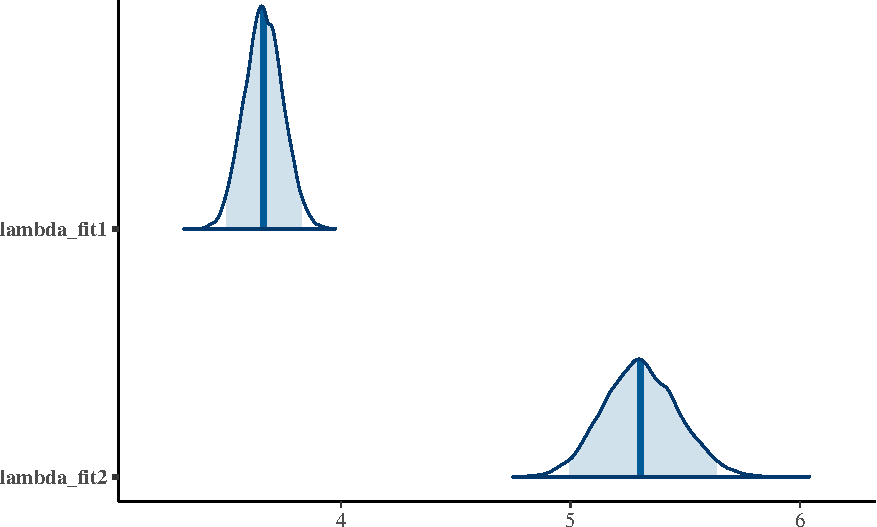
\includegraphics{046_ppc_files/figure-latex/unnamed-chunk-37-1} \end{center}

Rifacciamo i grafici esaminati in precedenza (e alcuni altri), ma questa volta eatraendo \(y^{rep}\) da \texttt{fit2}:

\begin{Shaded}
\begin{Highlighting}[]
\NormalTok{y\_rep2 }\OtherTok{\textless{}{-}} \FunctionTok{as.matrix}\NormalTok{(stanfit2, }\AttributeTok{pars =} \StringTok{"y\_rep"}\NormalTok{)}
\FunctionTok{ppc\_hist}\NormalTok{(y, y\_rep2[}\DecValTok{1}\SpecialCharTok{:}\DecValTok{8}\NormalTok{, ], }\AttributeTok{binwidth =} \DecValTok{1}\NormalTok{)}
\end{Highlighting}
\end{Shaded}

\begin{center}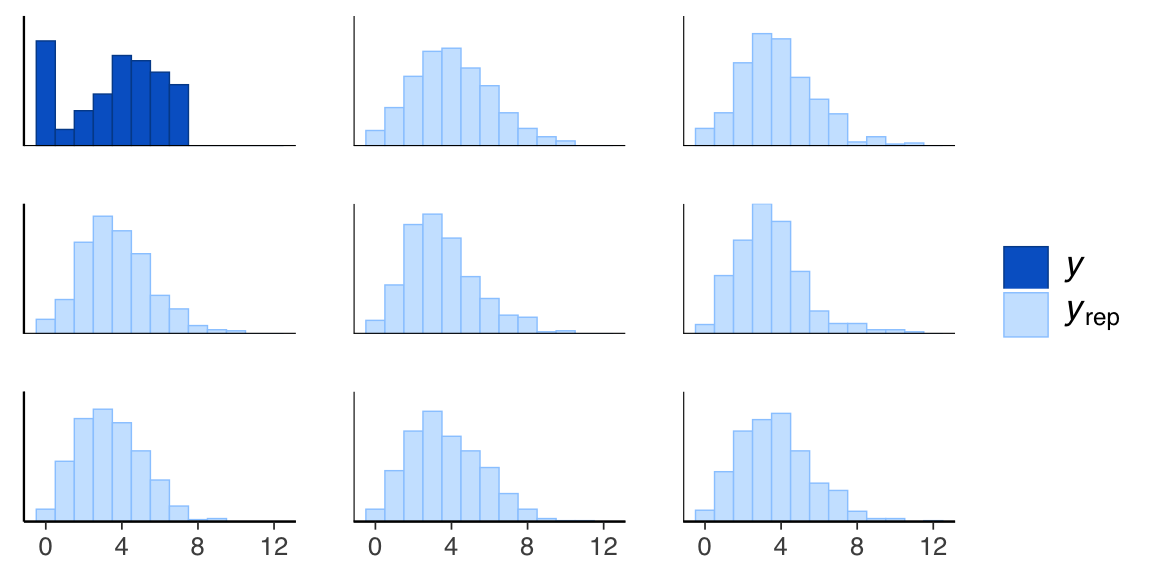
\includegraphics{046_ppc_files/figure-latex/unnamed-chunk-38-1} \end{center}

\noindent
In questo caso la distribuzione di \(y^{rep}\) è molto simile alla distribuzione di \(y\).

\begin{Shaded}
\begin{Highlighting}[]
\FunctionTok{ppc\_dens\_overlay}\NormalTok{(y, y\_rep2[}\DecValTok{1}\SpecialCharTok{:}\DecValTok{50}\NormalTok{, ])}
\end{Highlighting}
\end{Shaded}

\begin{center}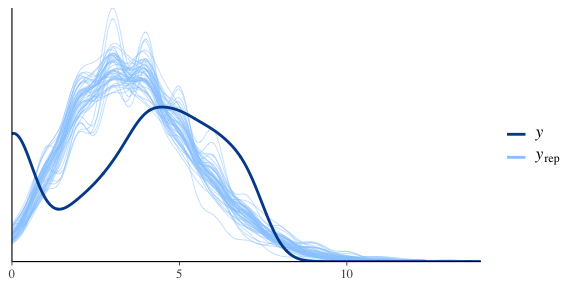
\includegraphics{046_ppc_files/figure-latex/unnamed-chunk-39-1} \end{center}

\begin{Shaded}
\begin{Highlighting}[]
\FunctionTok{ppc\_stat}\NormalTok{(y, y\_rep2, }\AttributeTok{stat =} \StringTok{"prop\_zero"}\NormalTok{)}
\end{Highlighting}
\end{Shaded}

\begin{center}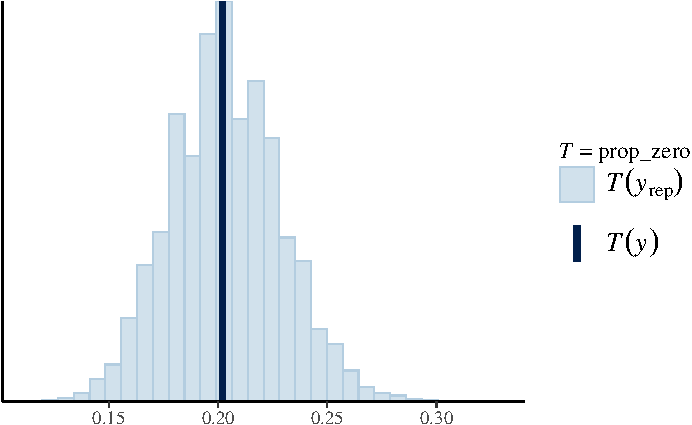
\includegraphics{046_ppc_files/figure-latex/unnamed-chunk-40-1} \end{center}

\begin{Shaded}
\begin{Highlighting}[]
\FunctionTok{ppc\_stat\_2d}\NormalTok{(y, y\_rep2, }\AttributeTok{stat =} \FunctionTok{c}\NormalTok{(}\StringTok{"mean"}\NormalTok{, }\StringTok{"sd"}\NormalTok{))}
\end{Highlighting}
\end{Shaded}

\begin{center}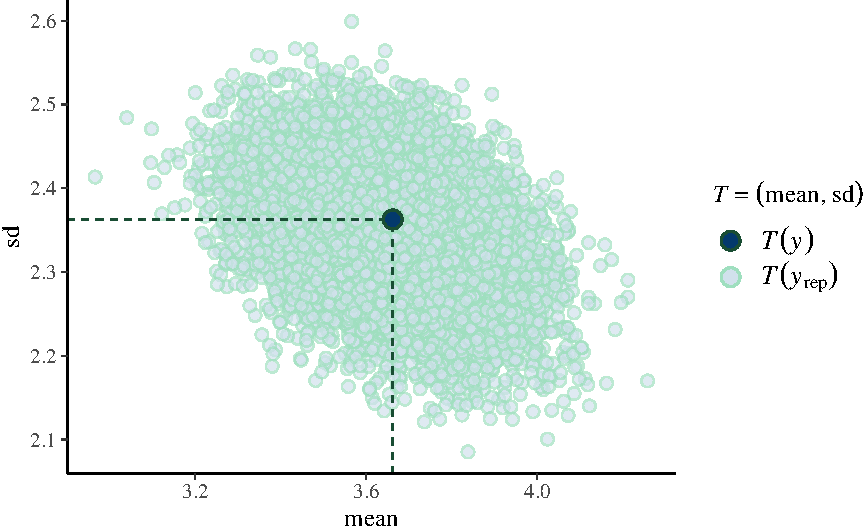
\includegraphics{046_ppc_files/figure-latex/unnamed-chunk-41-1} \end{center}

In conclusione, l'accuratezza predittiva del modello ``hurdle'' è chiaramente migliore di quella del modello di Poisson.

\hypertarget{considerazioni-conclusive}{%
\section*{Considerazioni conclusive}\label{considerazioni-conclusive}}
\addcontentsline{toc}{section}{Considerazioni conclusive}

Questo capitolo abbiamo discusso i controlli predittivi a posteriori. A questo proposito è necessario notare un punto importante: i controlli predittivi a posteriori, quando suggeriscono un buon adattamento del modello alle caratterische dei dati previsti futuri \(y^{rep}\), non forniscono una forte evidenza della capacità del modello di generalizzarsi a nuovi campioni di dati. Infatti, una tale evidenza sulla generalizzabilità del modello può essere solo fornita da studi di \emph{cross-validation}, ovvero da studi nei quali viene utilizzato un \emph{nuovo} campione di dati. D'altra parte, invece, se i PPC mostrano un cattivo adattamento del modello ai dati previsti futuri, questo fornisce una forte evidenza di una errata specificazione del modello.

  \bibliography{refs.bib,book.bib,packages.bib}

\end{document}
